\documentclass[conference]{IEEEtran}
\usepackage[T1]{fontenc}
\usepackage{microtype}
\usepackage{amsmath,amssymb}
\usepackage{graphicx,booktabs,array}
\usepackage{placeins,balance}
\usepackage{cite}
\usepackage[hidelinks]{hyperref}
\usepackage{xurl}
\setlength{\emergencystretch}{1.5em}
\renewcommand{\arraystretch}{1.08}
\title{Rebalancing Uneven Visual Data:\\Feature Equalization, Sampling, and Synthetic Images}
\author{\IEEEauthorblockN{Savannah Shannon, Kishor Datta Gupta, and Roy George}}
\begin{document}
\maketitle
\begin{abstract}
A biodiversity team may have thousands of photographs of common species and only a few of rare ones. Resampling, feature regularization, and generated images each offer a possible response, but improving a component need not improve the strongest complete pipeline. We first study feature equalization (EQ) under natural sampling with inverse-frequency loss weights and class-uniform sampling with unweighted loss. Across two frozen encoders and five ImageNet, CIFAR-100, and iNaturalist conditions, 80 tuning and 720 final fits support 30 planned contrasts over 12 paired seeds. EQ improves 18 of 20 encoder--sampler--condition cells, yet harms both encoders under natural sampling on CIFAR-100 LT100 ($-0.738$ and $-0.882$ macro-F1 points). A post-hoc analysis finds sharply different rare-class EQ eligibility, and 48 additional DeiT fits preserve the adverse natural-sampling direction across three split/rank configurations. A separate post-hoc experiment adds 35,223 generated images in three nested doses, with 192 fits and class-count-matched duplicate-real controls. Generated images help at every dose, but their advantage over duplication shrinks from 1.802 to 0.281 points for DeiT-S and from 2.474 to 1.040 for DINOv2-S as deficits are filled. Absolute synthetic scores show little additional gain at the largest dose under a fixed 1,950-update fitting budget. The original calibrated cross-entropy pipeline remains higher than these synthetic means, under different seeds and decision rules. The findings support evaluating sampling, prediction rules, and synthetic content together; they do not establish a universal synthetic-data limit or a causal mechanism for EQ.
\end{abstract}
\begin{IEEEkeywords}
long-tailed recognition, class imbalance, feature equalization, synthetic data, matched controls
\end{IEEEkeywords}

\section{Introduction}
Consider a biodiversity team sorting photographs submitted by volunteers. Familiar birds and flowers appear often, while a seldom-observed species may have only a few labeled images. A classifier could reduce the team's sorting effort, yet a good overall score would offer little reassurance if the system repeatedly missed less common species. Before choosing a training procedure, the team faces several practical decisions: how often should a rare example be sampled, how strongly should its errors be weighted, should the learned features be encouraged to form clearer class groups, and could generated images supply useful additional examples?

This example motivates the study; it is not an observed deployment. Naturally imbalanced collections such as iNaturalist provide a relevant benchmark setting \cite{vanhorn2018,inat2018}, while controlled thinning of object datasets lets us vary training support more deliberately. Neither setting, by itself, establishes how a system would behave in a conservation workflow. The immediate research question is narrower: when we add the same feature-equalization treatment to otherwise matched training procedures, does it help consistently?

EQ, as implemented here, encourages examples of the same class to cluster and eligible class centers to separate in the trainable adapter's feature space. Its contribution depends on which classes occur together in a minibatch. That creates a reason to examine EQ alongside sampling. We compare natural sampling with inverse-frequency loss weights against class-uniform sampling with unweighted loss. At a fixed model, both target the same expected class-balanced classification objective. Their batches and optimization trajectories can still differ.

We turn EQ off and on under each sampler, use two frozen pretrained encoder packages, and evaluate five conditions: native and study-specific LT100 versions of ImageNet-1K and CIFAR-100, plus naturally imbalanced iNaturalist 2018. Natural cross-entropy and Balanced Softmax serve as additional controls. All 720 final fits use the same 50-epoch schedule and 12 paired seeds, with learning-rate selection and calibration separated from the final evaluation.

The contribution is an empirical characterization of this fixed treatment under a controlled protocol. We ask whether its direction and magnitude persist across samplers, data conditions, and encoder packages, and whether gains within the factorial comparison translate into a stronger complete pipeline. The answer is qualified. EQ has positive mean effects in most tested cells, but it hurts both encoder packages under natural sampling on CIFAR-100 LT100. In addition, the calibrated cross-entropy control has higher mean macro-F1 than the four factorial arms on both artificial-tail conditions. We report these adverse outcomes, the complete contrast family, and the evaluation limits together.


After the primary study was completed, we examined the CIFAR LT100 direction change through retained eligibility and gradient diagnostics, an explicitly exploratory sampler-by-EQ contrast family, and 48 further DeiT fits varying split/rank and two treatment settings. We then tested a different intervention: generated images compared with duplicate-real controls at matched class counts and a fixed fitting budget, using 192 fits. These follow-ups answer narrower questions on already used test data; we report them separately from the original planned evidence. Their shared practical lesson is that balancing counts, changing a regularizer, and improving a prediction pipeline are related but distinct objectives.

\section{Background and Related Work}
Long-tailed recognition addresses unequal support across classes. Liu et al. introduced ImageNet-LT as part of an open long-tailed recognition framework \cite{liu2019}. The iNaturalist work documents a complementary challenge: visually similar species with naturally unequal image counts \cite{vanhorn2018}. Our artificial ImageNet LT100 condition is generated within the present protocol and is distinct from the published ImageNet-LT split. All tasks here use a fixed known class set; we do not evaluate recognition of unseen species or open-set detection.

Rebalancing can act through representation learning, sampling, loss weighting, or the prediction rule. Kang et al. separate representation and classifier learning \cite{kang2020}. Class-balanced loss uses an effective-number formulation \cite{cui2019}, and logit adjustment accounts for label frequencies in training or prediction \cite{menon2021}. Balanced Softmax incorporates training counts into the classification loss \cite{ren2020}. Our controls use ordinary natural cross-entropy with a development-selected logit offset and the Balanced Softmax loss. We do not implement the meta-sampler from Balanced Meta-Softmax or reproduce each cited paper's full training protocol.

DeiT provides a supervised pretrained transformer \cite{touvron2021}; DINOv2 provides representations learned through self-supervised pretraining \cite{oquab2023}. We keep both backbones frozen and train the same adapter structure on their features. Their contrast is a comparison of pretrained packages: pretraining data, training objective, patch geometry, and other model details differ. It cannot identify a causal advantage of self-supervision or architecture. The EQ objective below is the exact regularizer evaluated in this study; the term does not imply equivalence to covariance alignment or other feature regularizers.


Recent work also cautions against assuming that more adaptation is always better. LIFT reports that heavy fine-tuning of foundation models can harm tail classes and develops lightweight adaptation \cite{shi2024}. Our fixed cached-feature adapter differs from that method and is not a reproduction of its benchmark protocol. ProCo explicitly addresses inadequate class coverage in contrastive minibatches by estimating class distributions across batches \cite{du2024}. Thus, rare-class pair coverage is an established concern; our contribution is to measure eligibility and response for the particular EQ objective and sampling procedures tested here.

Synthetic-data research separates generation quality from downstream utility. CBDM studies diversity and fidelity losses when diffusion models are trained on imbalanced sources \cite{qin2023}. DiffuLT trains its generator using only the target long-tail data, without external pretrained weights \cite{shao2024}; our off-the-shelf SD-Turbo generator uses external pretraining. SynBalance studies quantity, diversity, recognizability, and domain gap together \cite{jiang2025}, while Decision Boundary-aware Generation targets informative near-boundary examples \cite{yang2026}. We do not reproduce these methods or claim to outperform them. The present follow-up isolates a simpler operational question: whether unfiltered, fixed-prompt synthetic images improve on count-matched repetition under a fixed number of adapter updates. Its limitations cannot be generalized to generators trained or filtered for different objectives.

\section{Study Design}
\subsection{A matched sampling comparison}
Let the fitting set contain $N$ rows in $C$ classes, with class counts $n_c>0$. For a per-example cross-entropy loss $\ell_i$, the balanced target is
\begin{equation}
R_{\mathrm{bal}}=\frac{1}{C}\sum_{c=1}^{C}\frac{1}{n_c}\sum_{i:y_i=c}\ell_i.
\label{eq:balanced}
\end{equation}
Natural sampling draws fitting rows uniformly with replacement and weights each loss by $N/(Cn_{y_i})$. Class-uniform sampling draws a row with probability $1/(Cn_{y_i})$ and leaves its loss unweighted. In either case we take an arithmetic minibatch mean. These are unbiased estimators of Eq.~\eqref{eq:balanced} at a fixed model. Matching that expectation does not match gradient variance, batch composition, clipping, or the trajectory of an adaptive optimizer.

The primary factorial crosses the two samplers with EQ off/on. We denote its four cells by N0, N1, U0, and U1, where N and U identify natural and class-uniform sampling. The additional CE control uses natural sampling and unweighted cross-entropy. The BS control uses natural sampling and the Balanced Softmax loss, $\mathrm{CE}(z_i+\log n,y_i)$, for logits $z_i$. Thus, CE and BS are practical pipeline comparisons rather than additional EQ-factorial cells.

\subsection{The feature-equalization treatment}
The adapter produces a vector $h_i$ for classification. EQ uses $u_i=h_i/\max\{\|h_i\|_2,10^{-12}\}$, the implementation's numerically stabilized normalization. For a minibatch $B$, let $B_c=\{i\in B:y_i=c\}$ and let $\mathcal E=\{c:|B_c|\geq2\}$ contain the eligible classes. With $K=|\mathcal E|$ and class center $\mu_c=|B_c|^{-1}\sum_{i\in B_c}u_i$, define
\begin{align}
W_B&=\frac{1}{K}\sum_{c\in\mathcal E}\frac{1}{|B_c|}\sum_{i\in B_c}\|u_i-\mu_c\|_2^2,\\
A_B&=\frac{2}{K(K-1)}\sum_{\substack{c<d\\c,d\in\mathcal E}}\|\mu_c-\mu_d\|_2^2,\quad K\geq2,\\
L_{\mathrm{EQ}}&=W_B-A_B.
\label{eq:eq}
\end{align}
For $K=1$, we use $A_B=0$; for $K=0$, the complete EQ loss is zero. Eligibility counts sampled occurrences, so two occurrences may come from replacement draws of the same image. The penalty adds compactness within each eligible class and rewards separation between eligible centers. It does not guarantee better rare-class recognition.

N1 and U1 minimize their classification loss plus $0.05L_{\mathrm{EQ}}$ during epochs 41--50. The penalty is inactive during epochs 1--40 and throughout N0 and U0. This fixed coefficient and onset define the treatment; we do not tune them separately for each dataset or sampler.

\subsection{Data, exclusions, and partitions}
ImageNet uses the ILSVRC 2012 training source and labeled validation source \cite{russakovsky2015}. CIFAR-100 uses its official training and test sources \cite{krizhevsky2009}. iNaturalist uses the 2018 competition release \cite{inat2018}. We call the official labeled validation or test source the \emph{confirmation set}, because it is reserved for evaluation after the study's selection choices are frozen. Table~\ref{tab:data} gives the actual partitions, rather than nominal fractions alone.

\begin{table*}[t]
\centering\footnotesize
\caption{Actual partition sizes. Source train is the official training inventory before exclusions; excluded counts apply to that source and are repeated across its two conditions. LT100 only thins the fitting pool. Confirmation retains every official labeled evaluation row. Classes and development/confirmation rows are shared by both encoders.}
\label{tab:data}
\begin{tabular}{lrrrrrrr}
\toprule
Condition & Classes & Source train & Excluded & Fit & Tune & Calibrate & Confirm. \\
\midrule
ImageNet native & 1,000 & 1,281,167 & 12,497 & 1,142,920 & 62,875 & 62,875 & 50,000 \\
ImageNet LT100 & 1,000 & 1,281,167 & 12,497 & 250,594 & 62,875 & 62,875 & 50,000 \\
CIFAR native & 100 & 50,000 & 33 & 44,995 & 2,486 & 2,486 & 10,000 \\
CIFAR LT100 & 100 & 50,000 & 33 & 9,777 & 2,486 & 2,486 & 10,000 \\
iNaturalist 2018 & 8,142 & 437,513 & 3 & 395,078 & 21,216 & 21,216 & 24,426 \\
\bottomrule
\end{tabular}
\end{table*}

The duplicate policy was fixed before extraction and fitting. It preserves all official confirmation rows and their original labels, including conflicting-label duplicate groups. Training images with identical decoded RGB pixels, including dimensions, to any confirmation image are excluded. For training-only duplicate groups, all members with conflicting labels are excluded; a same-label group retains its lexicographically first sample ID. Original source inventories and exclusions are retained. These checks address declared source overlap; they cannot establish independence from pretrained-model data.

After exclusions, a fixed split seed of 20261016 allocates nominally 5\% of each class to tuning and 5\% to calibration. Classes with at least three eligible rows reserve at least one row for each development role and one for fitting. Classes with one or two rows remain fit-only. Native conditions retain the remaining fitting pool.

For LT100, a seeded permutation assigns class ranks $r_c\in\{0,\ldots,C-1\}$. If the largest remaining class has $m$ fitting rows, the target is $\max\{1,\lfloor m100^{-r_c/(C-1)}\rfloor\}$, capped by the class's available pool. The resulting CIFAR fitting supports range from 4 to 450 per class, and ImageNet supports range from 11 to 1,165. LT100 describes this intended exponential thinning, not a guarantee of an exact realized ratio of 100. Native and LT100 conditions share development and confirmation sets within each source, so they are related conditions rather than independent dataset replications.

\subsection{Representations and optimization}
We use the pinned model packages \nolinkurl{deit_small_patch16_224.fb_in1k} and \nolinkurl{vit_small_patch14_dinov2.lvd142m}. Both produce 384-dimensional pooled features under the common input transform: bicubic shorter-side resize to 256, a central $224\times224$ crop, and ImageNet channel normalization, with no augmentation. One float16 frozen-feature cache per encoder and source is shared across matched arms. Means and standard deviations are fitted on fitting rows alone.

The float32 trainable adapter applies LayerNorm, a $384\rightarrow256$ linear projection, GELU, and LayerNorm, followed by a linear classifier. Dropout is zero. Classification uses the adapter output before EQ normalization. The backbone is frozen throughout; the experiment tests adaptation of pretrained features, not end-to-end representation learning.

All fits use AdamW \cite{loshchilov2019}, weight decay 0.01, global gradient clipping at 1, 10\% linear warmup, and cosine learning-rate decay. An epoch consists of $\lceil N/256\rceil$ full replacement-sampled batches of 256. Every fit therefore receives $50\lceil N/256\rceil$ updates; an epoch does not mean that every distinct fitting image is visited. We retain the final epoch rather than select a checkpoint on confirmation performance.

Each encoder--condition context tunes two learning rates, $0.001$ and $0.003$, using seed 901. The mean raw tuning macro-F1 of N0 and U0 selects one shared rate for N0, N1, U0, and U1. CE and BS select their own rates on the same tuning role. Four EQ-off/control arms at two rates yield eight tuning fits per context, or 80 across ten contexts. Six final arms at seeds 10--21 yield 72 fits per context, or 720 overall. All four factorial cells selected 0.001 in every context; Appendix~\ref{app:settings} records control-rate exceptions.

\subsection{Decision rules and the primary endpoint}
For CE only, calibration selects $\tau\in\{0,0.05,\ldots,2\}$ to maximize calibration macro-F1 under the prediction rule
\begin{equation}
\hat y(x)=\arg\max_c\{z_c(x)-\tau\log(n_c/N)\}.
\end{equation}
Ties use the first maximizing grid value. The four factorial arms and BS use the fixed unadjusted readout ($\tau=0$). Consequently, an EQ contrast within a sampler is unaffected by calibration selection, while CE's reported score includes its separately chosen decision rule.

The primary endpoint is macro-F1 on confirmation rows. We compute F1 separately for every declared class and average equally over classes, assigning zero when the denominator is zero. Equal class weighting does not make the metric independent of evaluation prevalence. Top-1, top-5, macro precision, macro recall, and class-level metrics are retained. Head, middle, and tail thirds are defined by descending fitting support with label order breaking ties. These slices are descriptive, especially on near-balanced native CIFAR-100.

\subsection{Planned contrasts and uncertainty}
For each encoder, sampler, and condition, we subtract the EQ-off macro-F1 from EQ-on within each seed. We report the mean difference in percentage points (pp). For each sampler we also subtract the DeiT EQ effect from the DINOv2 effect. The four EQ effects and two encoder interactions yield six planned contrasts per condition and 30 overall. The encoder interactions compare EQ responses between pretrained packages; they do not isolate the effect of architecture or supervision. A formal sampler-by-EQ contrast is not part of this planned family.

Pointwise 95\% paired $t$ intervals use the 12 seed differences and 11 degrees of freedom. Exact two-sided sign-flip tests enumerate all $2^{12}$ sign assignments of the paired differences, using absolute mean difference as the statistic. Their interpretation requires appropriate sign exchangeability or symmetry; matching seed labels does not itself establish that assumption. Holm adjustment controls each six-contrast condition family under valid input $p$-values \cite{holm1979}; correction across all 30 is a sensitivity analysis. Intervals are not simultaneous confidence intervals. The minimum two-sided unadjusted $p$-value is $2/4096$, a resolution limit rather than a power guarantee.

The seeds vary initialization and sampling within fixed partitions, pretrained models, and selected configurations. They do not sample new datasets, class-rank permutations, development splits, or pretraining runs. All uncertainty statements below have that conditional scope.

\subsection{Execution and evidence checks}
All 800 tuning/final fits completed the declared budgets before confirmation. A separately implemented full-grid audit checked source and cache bindings, regenerated partitions and scalers, validated checkpoints and optimizer budgets, reproduced tuning scores and learning-rate selection, and checked bound artifact hashes. A separate provenance check covered four recorded GPU attempts, including interrupted attempts and their resumptions. The training grid was then globally sealed before confirmation. Analysis recomputed calibration choices and metrics from saved predictions. These are checks of execution and retained evidence, not independent retraining or external replication. The retained export was independently byte-verified after transfer off the experiment machine.

\FloatBarrier
\section{Results}
\begin{figure*}[t]
\centering
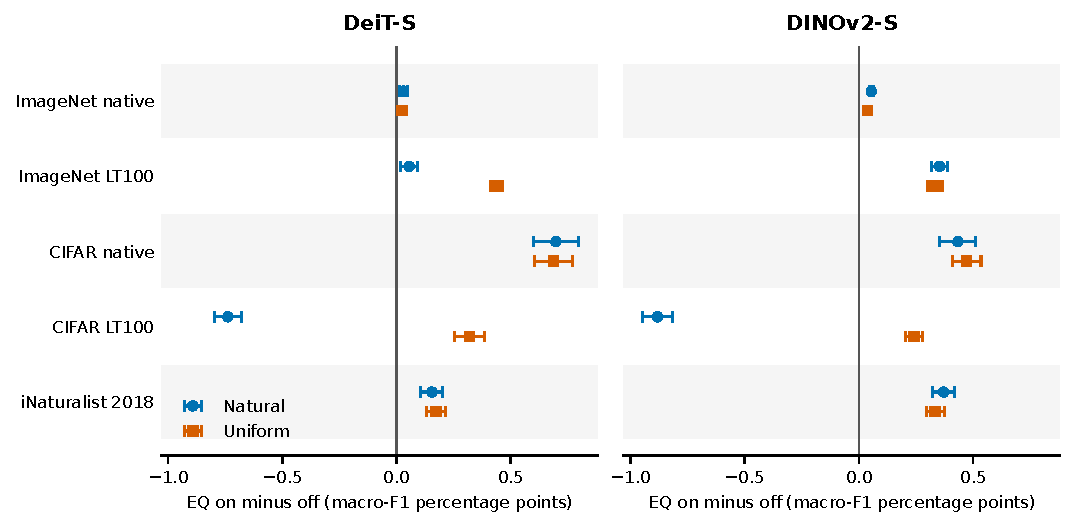
\includegraphics[width=\textwidth]{eq_effects.pdf}
\caption{All 20 planned EQ-on/off mean effects. Points and bars show mean paired differences and pointwise 95\% paired $t$ intervals over 12 optimization seeds, conditional on fixed partitions and selected models. Natural sampling uses inverse-frequency loss weights; class-uniform sampling uses unweighted loss. The same horizontal scale is used for both encoders. Full multiplicity-adjusted results, including encoder interactions, appear in Appendix~\ref{app:contrasts}.}
\label{fig:effects}
\end{figure*}
\subsection{EQ's direction depends on the tested setting}
Figure~\ref{fig:effects} shows all 20 EQ-on/off effects. Eighteen are positive. The two negative effects both occur on CIFAR-100 LT100 under natural sampling: $-0.738$ pp for DeiT-S (95\% CI $[-0.797,-0.679]$) and $-0.882$ pp for DINOv2-S ($[-0.948,-0.815]$). Under class-uniform sampling, the corresponding effects are $+0.318$ pp ($[+0.252,+0.385]$) and $+0.241$ pp ($[+0.205,+0.277]$). Each of these four planned contrasts has within-condition Holm-adjusted $p=0.0029$ and across-30 adjusted $p=0.0146$. We describe the observed direction change without treating it as a separately tested sampler interaction.



On ImageNet LT100, class-uniform EQ improves macro-F1 by $+0.438$ pp for DeiT-S and $+0.333$ pp for DINOv2-S. Natural-sampling effects are $+0.055$ and $+0.353$ pp. On naturally imbalanced iNaturalist, the four effects range from $+0.154$ to $+0.371$ pp. Native CIFAR effects range from $+0.433$ to $+0.698$ pp. These positive results establish the treatment's behavior in the tested settings without making it a general remedy for rarity.

Native ImageNet illustrates why effect size matters alongside statistical evidence. Its four EQ effects are positive but only $+0.024$ to $+0.054$ pp. A small and repeatable seed-conditional difference can have an adjusted $p$-value below 0.05 while offering little practical improvement. No minimum useful effect or equivalence margin was specified, so we do not label these differences practically meaningful or equivalent to zero.

\subsection{Encoder responses and multiplicity}
Appendix~\ref{app:contrasts} reports every planned contrast. Twenty-nine of 30 have within-condition Holm-adjusted $p\leq0.05$; 28 remain below that threshold after correction across all 30. This count includes encoder interactions and should not be read as 29 beneficial treatments. For example, ImageNet LT100's encoder interaction is positive under natural sampling ($+0.298$ pp) and negative under class-uniform sampling ($-0.104$ pp), reflecting differences in the magnitude of EQ effects.

The native ImageNet class-uniform encoder interaction has within-condition adjusted $p=0.0488$ but across-30 adjusted $p=0.0977$. The CIFAR LT100 class-uniform encoder interaction has within-condition adjusted $p=0.0854$ and an interval spanning zero. We retain these results rather than describe the encoder response as uniformly different. A displayed interval endpoint rounded to $+0.000$ should not be used to infer an exact zero boundary; inference uses the retained unrounded values.

\subsection{A component gain does not settle the pipeline choice}
Table~\ref{tab:arms} gives the 60 arm means. On CIFAR LT100, CE with its selected logit offset reaches 66.616\% macro-F1 for DeiT-S and 77.972\% for DINOv2-S, compared with 60.105\% and 71.535\% for U1. On ImageNet LT100 the corresponding CE scores are 74.238\% and 67.711\%, compared with U1's 72.710\% and 64.803\%. CE also exceeds N0, N1, and U0 in these four encoder--condition contexts.

\begin{table*}[t]
\centering\footnotesize
\caption{Mean confirmation macro-F1 (\%) across 12 seeds. N0/N1 use natural sampling with inverse-frequency loss weights and EQ off/on; U0/U1 use class-uniform sampling and EQ off/on. CE includes a calibration-selected logit offset; BS uses the Balanced Softmax loss. These are descriptive complete-pipeline means. Paired uncertainty for the planned contrasts appears in the figure and appendix.}
\label{tab:arms}
\begin{tabular}{llrrrrrr}
\toprule
Condition & Encoder & N0 & N1 & U0 & U1 & CE & BS \\
\midrule
ImageNet native & DeiT-S & 76.493 & 76.523 & 76.464 & 76.488 & 76.399 & 76.408 \\
ImageNet native & DINOv2-S & 77.633 & 77.687 & 77.602 & 77.640 & 77.645 & 77.682 \\
\addlinespace[2pt]
ImageNet LT100 & DeiT-S & 72.238 & 72.293 & 72.273 & 72.710 & 74.238 & 73.251 \\
ImageNet LT100 & DINOv2-S & 64.323 & 64.676 & 64.470 & 64.803 & 67.711 & 66.039 \\
\addlinespace[2pt]
CIFAR native & DeiT-S & 75.709 & 76.406 & 75.581 & 76.269 & 75.711 & 75.711 \\
CIFAR native & DINOv2-S & 85.071 & 85.504 & 85.020 & 85.491 & 85.073 & 85.068 \\
\addlinespace[2pt]
CIFAR LT100 & DeiT-S & 59.759 & 59.021 & 59.786 & 60.105 & 66.616 & 63.780 \\
CIFAR LT100 & DINOv2-S & 71.476 & 70.595 & 71.294 & 71.535 & 77.972 & 75.437 \\
\addlinespace[2pt]
iNaturalist 2018 & DeiT-S & 34.054 & 34.209 & 34.838 & 35.011 & 35.119 & 34.556 \\
iNaturalist 2018 & DINOv2-S & 59.832 & 60.203 & 60.514 & 60.848 & 60.264 & 59.759 \\
\bottomrule
\end{tabular}
\end{table*}

These are descriptive comparisons of complete pipelines. CE changes the training objective and has a selected decision offset; controls can also select a different learning rate. Their ranking does not isolate the contribution of the offset, loss, or sampling alone. Nor is CE best in every context: on iNaturalist DINOv2-S, U1 averages 60.848\% versus CE's 60.264\%. A positive EQ component effect and a preference among complete pipelines answer different questions.

\subsection{Secondary metrics add context}
As a descriptive check, natural-sampling EQ on CIFAR LT100 changes mean tail-third F1 by $-1.490$ pp for DeiT-S and $-1.870$ pp for DINOv2-S; macro recall changes by $-0.652$ and $-0.744$ pp. These averages come from the same paired seeds and have no separate multiplicity-adjusted inference here. They do not show that every rare class worsens. Class-specific support, precision, recall, and error costs would be needed to judge a use such as the biodiversity example.


\FloatBarrier
\section{Post-hoc EQ Follow-up}
\label{sec:eqfollow}
The adverse CIFAR LT100 result prompted two additional questions: which classes actually participate in EQ, and does the observed direction persist under a few alternative settings? These analyses were designed after the primary results were known. They do not enlarge or revise the original 30-contrast family, and they reuse a test set already evaluated in the primary study.

\subsection{Eligibility and retained gradient diagnostics}
For independent replacement draws in a batch of size $B$, let $p_c$ be the probability that a draw belongs to class $c$. Then
\begin{equation}
\Pr(|B_c|\geq2)=1-(1-p_c)^B-Bp_c(1-p_c)^{B-1}.
\end{equation}
Here $p_c=n_c/N$ under natural sampling and $p_c=1/C$ under uniform sampling. Two occurrences need not be two different images. If the $n_c$ source images are equally likely within class, the probability of at least two distinct images is
\begin{equation}
1+(n_c-1)(1-p_c)^B-n_c(1-p_c+p_c/n_c)^B.
\end{equation}
These sampling probabilities describe opportunities for EQ to act, not its effect on a classifier's errors.

We checked 480 immutable factorial training histories against their export inventory and summed the retained class-level counters over epochs 41--50. Eligibility vectors agreed exactly within all 240 EQ-off/on seed pairs. For the CIFAR LT100 tail third, the mean occurrence-eligibility rate was 0.0317 with natural sampling and 0.7291 with uniform sampling. Requiring two distinct source images reduced these rates to 0.0291 and 0.6927. Figure~\ref{fig:followeq}(a) compares the retained rates with the sampling formula. The increase therefore reflects more opportunities involving distinct rare images as well as replacement duplicates.

Retained gradient diagnostics add scale information, but are sampled steps rather than a record of every update. On CIFAR LT100, the median across run medians of the weighted EQ-to-classification adapter-gradient norm ratio was 0.836 under natural sampling versus 0.505 under uniform sampling for DeiT-S; the DINOv2-S values were 1.169 and 0.766. Each encoder--sampler summary contains 120 logged ratios. These norms omit gradient direction, clipping's realized effect, and AdamW's state-dependent rescaling. Neither these ratios nor eligibility differences establish a causal explanation of the accuracy change.

We also evaluated the previously unplanned sampler-by-EQ difference, $(U1-U0)-(N1-N0)$, for all ten encoder--condition contexts. On CIFAR LT100 it was $+1.056$ pp for DeiT-S (pointwise 95\% CI $[+0.956,+1.156]$) and $+1.123$ pp for DINOv2-S ($[+1.033,+1.212]$). Both have exact sign-flip $p=0.00049$ and Holm-adjusted $p=0.0049$ within this \emph{separate exploratory ten-comparison family}. Appendix~\ref{app:posthoc} reports the entire family, including nonsignificant outcomes. This formalizes the observed response difference without retrospectively calling it a planned primary test.

\begin{figure*}[t]
\centering
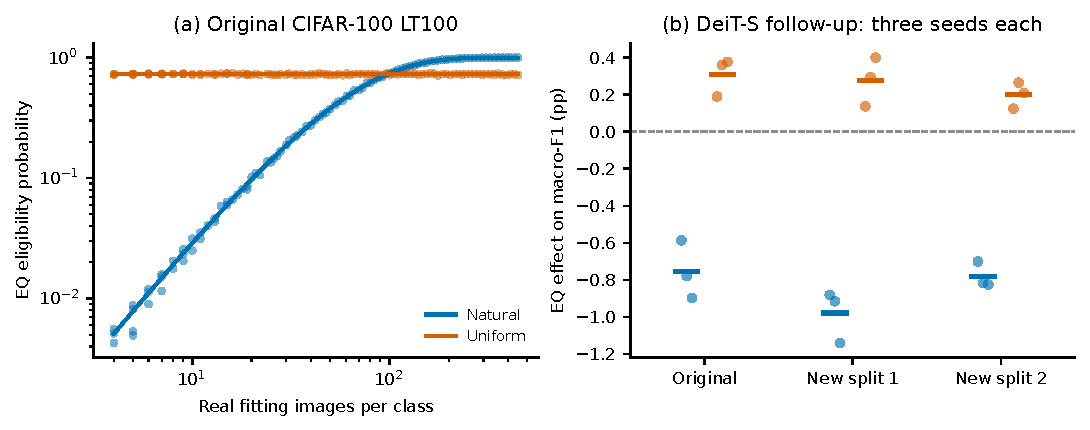
\includegraphics[width=\textwidth]{eq_followup_diagnostics.pdf}
\caption{Exploratory EQ evidence. (a) Lines are theoretical occurrence-eligibility probabilities; dots are retained late-phase rates over the original 12 seeds. The CIFAR class counts and sampling counters are identical across the two encoders. (b) Each dot is an individual paired EQ effect in the new DeiT-S follow-up; short bars mark three-seed means. These three split/rank configurations do not establish population-level robustness or a causal mechanism.}
\label{fig:followeq}
\end{figure*}

\subsection{Split and treatment sensitivity: 48 additional fits}
We reused the verified frozen DeiT-S CIFAR cache for a separate local CPU study. The original split/rank seed 20261016 and two new seeds, 202611021 and 202611022, each crossed natural/uniform sampling with EQ off/on at training seeds 101--103, giving 36 fits. The new seeds jointly change development allocation and LT class ranks; their effects cannot be separated in this design. Twelve further fits on the original split tested a smaller coefficient ($0.01$ rather than $0.05$) and an earlier onset (epoch 26 rather than 41), each under both samplers and all three seeds. Each ablation reuses the original-split EQ-off comparison.

All 48 fits used 50 epochs, the fixed 0.001 learning rate, the original adapter and real-fit-only scaling, and the final checkpoint with $\tau=0$. No configuration was selected using the new test scores. All checkpoints were budget-checked and sealed before scoring all 10,000 official test rows. A fresh call to the original CPU evaluator reproduced every stored prediction and metric. The portable implementation's vectorized EQ passed value and gradient checks against the original expression; that does not establish bitwise equivalence to primary A100 training.

\begin{table}[t]
\centering\footnotesize
\caption{Exploratory DeiT-S EQ follow-up: mean paired EQ-on minus EQ-off macro-F1 (pp), three training seeds per row. New splits jointly change development allocation and LT class ranks. Ablations use the original split and reuse its EQ-off controls.}
\label{tab:eqfollow}
\begin{tabular}{lrr}
\toprule
Setting & Natural & Uniform \\
\midrule
Original, default & $-0.754$ & $+0.309$ \\
New split 1, default & $-0.978$ & $+0.277$ \\
New split 2, default & $-0.781$ & $+0.199$ \\
Original, $\lambda=0.01$ & $-0.156$ & $+0.044$ \\
Original, earlier onset & $-0.771$ & $+1.180$ \\
\bottomrule
\end{tabular}
\end{table}

The default natural-sampling effect remains negative in all three tested split/rank configurations, while the uniform-sampling effect remains positive (Table~\ref{tab:eqfollow}). Lowering the coefficient reduces both the natural-sampling loss and the uniform-sampling gain. Earlier onset gives a larger uniform-sampling gain on the original split, but does not remove the natural-sampling loss. These three-seed descriptions identify settings worth testing in a separately designed study; they neither identify an optimal setting nor supply a new confirmatory significance claim.

\section{Generated Images Under a Fixed Fitting Budget}
\label{sec:generated}
Sampling and regularization reorganize information already available to training. A team facing rare categories might instead ask a generator for additional examples. We tested that possibility in a separate post-hoc CIFAR-100 LT100 experiment: do generated pixels improve on repeating real fitting images when the class counts and optimizer budget match, and does filling more of the numerical deficit keep improving recognition?

\subsection{A nested image bank and matched duplicate controls}
We used the same 9,777-row real fitting partition, with a maximum of 450 rows in a class. A pinned SD-Turbo checkpoint \cite{sdturbo} produced one bank of 35,223 images, enough to fill every class's numerical deficit to 450. Generation used one fixed text prompt per class, deterministic per-image seeds, one inference step, guidance scale zero, and $512\times512$ output. Images were downsampled with bicubic interpolation to CIFAR's $32\times32$ resolution before the original encoder transform. There was no quality filter or recognition-score selection. Labels denote intended prompt categories; they are not independently verified semantic labels. The model revision, all prompts, and generation settings accompany the released protocol.

For dose $d\in\{0.1,0.5,1\}$, class $c$ receives $\lfloor d(450-n_c)\rfloor$ additional rows. Smaller doses use nested prefixes of the same generated bank. The total added rows are 3,480, 17,590, and 35,223. A paired duplicate-real control repeats only real fitting images to create the exact same class-count vector and pool label order at each dose. Real-only natural and class-uniform arms provide two further references. Generated-versus-duplicate contrasts therefore compare the supplied pixels/features while holding these reweighting and row-count consequences fixed. They do not isolate every possible effect of generator quality or external pretraining.

Each of the two encoders has eight conditions at 12 training seeds (101--112): 192 fits in total. All use unweighted cross-entropy, no EQ, no logit offset, the original 256-wide adapter, learning rate 0.001, and a scaler fitted only on the original real fitting rows. Crucially, every fit receives 50 rounds of 39 full replacement-sampled batches of 256: 1,950 AdamW updates. These are \emph{not} 50 full passes over each augmented pool. Larger pools consequently have fewer expected visits per row at the same total fitting budget. Generator and encoder computation are additional costs; equal adapter updates do not imply equal total computation.

Synthetic and duplicate conditions for a seed were assigned to the same GPU, with each condition distributed over four GPUs in groups of three seeds. All 192 checkpoints were validated and sealed before evaluating the unchanged 10,000 real test images. A fresh audit reproduced saved predictions, top-five indices, and metrics with the original A100 evaluator; it also checked generated image bytes, the exact-duplicate rule, augmented pools, scalers, and retained execution records. A CPU check found one fifth-ranked device-sensitive discrepancy; top-one predictions and aggregate metrics agreed. We therefore claim evaluator reproduction on the bound A100 runtime, not universal cross-device bitwise prediction equality. The image-containing archive was independently byte-verified after transfer and is retained privately.

\subsection{Benefits over duplicates, then diminishing returns}
The follow-up defined six synthetic-minus-duplicate macro-F1 contrasts before its own scoring. Table~\ref{tab:generated} gives all six, with paired $t$ intervals and exact sign-flip tests over 12 seeds, Holm-adjusted within this separate family. The test assumptions and seed-conditional interpretation from the primary study still apply. The design remains post-hoc relative to the already observed primary study and its test set.

\begin{table*}[t]
\centering\footnotesize
\caption{Generated-image follow-up: all six predefined synthetic-minus-duplicate comparisons. Scores are mean macro-F1 (\%) over 12 seeds; effects and pointwise paired 95\% intervals are in pp. Holm adjustment covers only this separate six-comparison family. Every cell receives 1,950 updates, unweighted CE, no EQ, and no logit adjustment.}
\label{tab:generated}
\begin{tabular}{llrrrrr}
\toprule
Encoder & Deficit filled & Duplicate & Synthetic & Difference & Pointwise 95\% CI & Holm $p$ \\
\midrule
DeiT-S & 10\% & 58.325 & 60.127 & $+1.802$ & $[+1.634,+1.970]$ & 0.0029 \\
DeiT-S & 50\% & 59.449 & 60.078 & $+0.629$ & $[+0.447,+0.810]$ & 0.0029 \\
DeiT-S & 100\% & 59.771 & 60.052 & $+0.281$ & $[+0.102,+0.460]$ & 0.0039 \\
DINOv2-S & 10\% & 69.723 & 72.197 & $+2.474$ & $[+2.380,+2.568]$ & 0.0029 \\
DINOv2-S & 50\% & 70.969 & 72.469 & $+1.500$ & $[+1.408,+1.592]$ & 0.0029 \\
DINOv2-S & 100\% & 71.404 & 72.444 & $+1.040$ & $[+0.846,+1.234]$ & 0.0029 \\
\bottomrule
\end{tabular}
\end{table*}

Generated images improve on matched duplicates at every tested dose. For DeiT-S, the advantage falls from $+1.802$ pp at 10\% deficit filling to $+0.281$ pp at full filling. For DINOv2-S it falls from $+2.474$ to $+1.040$ pp. This shrinking advantage partly reflects improvement of the duplicate control itself. Figure~\ref{fig:generated} shows both curves rather than treating the relative difference as a synthetic-score curve.

\begin{figure*}[t]
\centering
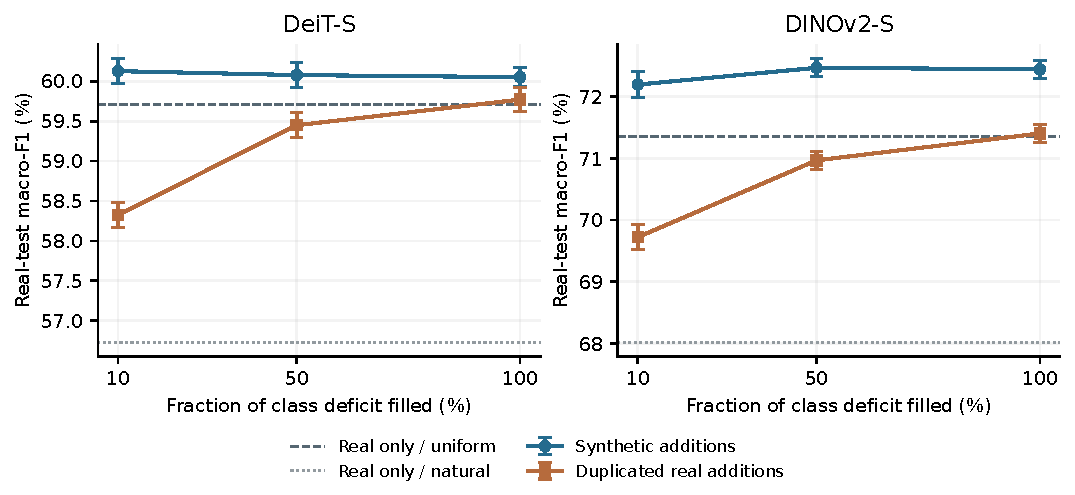
\includegraphics[width=\textwidth]{generated_dose_response.pdf}
\caption{Generated-image follow-up under 1,950 adapter updates per fit. Synthetic and duplicate-real pools have matched class counts at each dose; horizontal references show real-only natural and uniform sampling. Scores are 12-seed means on the same real test set. The six paired differences are reported in Table~\ref{tab:generated}. Flat-looking portions of these curves do not establish equivalence, an optimal dose, or a universal limit of synthetic data.}
\label{fig:generated}
\end{figure*}

Absolute synthetic scores also show limited further improvement in this regime. DeiT-S averages 60.127\%, 60.078\%, and 60.052\% across the three doses; DINOv2-S averages 72.197\%, 72.469\%, and 72.444\%. The descriptive 100\%-minus-50\% changes are $-0.026$ and $-0.025$ pp. No equivalence margin or adjusted dose-selection family was specified. These observations support \emph{diminishing returns under this fixed update budget}, not equality between doses or a general ceiling on generated data. Larger pools, fewer visits per row, and generator-specific properties all remain possible contributors.

The real-uniform controls average 59.714\% and 71.362\%, so the fully filled synthetic pools exceed them descriptively by 0.338 and 1.082 pp. Yet the primary study's calibrated CE pipeline reached 66.616\% and 77.972\% on this partition, substantially above every synthetic mean here. These are different seed sets and decision rules, not a matched test of generation against calibration. The follow-up establishes benefit over its duplicate controls; it does not establish the best overall pipeline or a gain beyond calibrated CE. All 16 condition means are retained in Appendix~\ref{app:generatedmeans}.

\subsection{What this experiment cannot resolve}
The generated-image result is conditional on one real split, one generator revision, one prompt per class, one generated bank, two frozen encoders, and three doses. Twelve fitting seeds do not measure variation across independent image banks. No exact decoded-pixel duplicates were found within the bank or against the full real CIFAR source; this does not exclude near-duplicates, generator/pretraining overlap, or incorrect prompt labels. We did not vary the training budget, audit semantic fidelity, or measure classwise diversity and domain gap. The experiment therefore cannot distinguish a fundamental information limit from insufficient fitting exposure, semantic errors, or a mismatch between synthetic and real images.

For the motivating biodiversity team, generating a larger folder would not by itself verify that rare species are represented faithfully. The present object-recognition evidence supports checking generated content against matched repetition controls and a strong calibrated baseline. It does not validate generated species labels or demonstrate benefit in a conservation workflow.

\section{Discussion and Limitations}
\subsection{What a practitioner can take from the comparison}
For a team deciding how to train on uneven data, the main finding is a dependence worth checking: the same EQ setting can behave differently with a different sampler. Testing the regularizer in isolation from the intended sampling procedure would miss the adverse natural-sampling result on CIFAR LT100. The controls add a second lesson: an improvement from adding EQ does not establish that the resulting pipeline is the strongest choice among those evaluated. The prediction rule and the reference pipeline deserve the same attention as the added regularizer.

The follow-up narrows the description without establishing the mechanism. Class eligibility and retained gradient norms differ under the two samplers, and changing the coefficient or onset changes the observed effect. However, these observations do not isolate eligibility from loss weighting, gradient direction, clipping, or AdamW's state. A targeted intervention that changes one proposed mediator while controlling the others is still needed. Similarly, the generated-image experiment measures useful additional content relative to duplicates, but does not identify which semantic or distributional properties produce that benefit.

\subsection{Limits of the data and representations}
Artificial tails change available training support within the same source collection. They do not recreate all causes of natural rarity, including collection bias, environmental change, or the difficulty of distinguishing related species. The primary study uses one LT100 class-rank permutation and shared source partitions. The two additional CIFAR split/rank configurations in the DeiT follow-up modestly broaden this check; three configurations do not characterize a population of possible long tails. iNaturalist supplies a natural imbalance, but its 24,426 confirmation images cover 8,142 species, leaving many class estimates sensitive to limited support. None of these benchmarks reproduces a particular field prevalence or workflow.

Pretraining limits the interpretation of encoder comparisons. DeiT's supervised pretraining already uses ImageNet labels, and thinning the downstream fitting pool does not erase that exposure. DINOv2's package differs in pretraining data and objective as well as model details. We therefore interpret ImageNet results as adaptation of existing representations and encoder interactions as package-level comparisons. We make no from-scratch, isolated architectural, or full-backbone-training claim.

\subsection{Limits of tuning, inference, and verification}
The primary grid fixes the EQ coefficient, its late onset, the adapter, one development split, and two learning-rate candidates. It does not determine the best EQ hyperparameters for each setting. Using a common learning rate in the factorial helps define the matched comparison, but results may differ under separately optimized treatments. Twelve seeds quantify a limited source of optimization variation. They do not support population-level uncertainty over new datasets or repeated development choices. Sign-flip assumptions and pointwise intervals remain relevant even when adjusted $p$-values are small.

The confirmation sets were protected from the current selection procedure, not from all historical research use or possible pretrained-data overlap. The scientific audit verified encoded source bytes, frozen annotations/manifests, and the declared artifact relationships. It did not independently reconstruct every ImageNet or iNaturalist label or decode every image anew. GPU provenance and received-byte verification support traceability without replacing an external scientific replication. We make no timing, energy, or deployment-cost ranking because a comparable isolated cost analysis has not been established.

\section{Conclusion}
The primary study shows that EQ's effect depends on the tested training procedure: gains dominate the grid, but natural-sampling EQ hurts both encoders on CIFAR LT100. Post-hoc diagnostics describe unequal opportunities for rare classes to participate, and a small split/treatment follow-up preserves the natural-sampling adverse direction. Generated images provide a separate benefit over count-matched duplication, with diminishing returns under a fixed adapter-update budget. Neither result establishes the strongest complete pipeline: calibrated CE remains a substantial reference, and no universal synthetic-data ceiling follows from one bank and budget. For a team working with uneven visual data, the useful comparison includes the sampling procedure, prediction rule, actual content of additional images, and the scope of the evidence.

\section*{Code and Result Availability}
The \href{https://github.com/savannahshannon/rebal/tree/vision-only-fullscale/vision_only}{REBAL vision-only branch} contains the original scientific code, the revised manuscript, per-seed numeric tables for the primary study and both follow-ups, complete comparison families, sanitized follow-up settings, and presentation-reproduction code. The primary 30, exploratory ten, and generated-image six comparison families are separate files. Source and generated images, credentials, and private operational metadata are excluded from the public release. Checkpoints, image-bearing follow-up evidence, and detailed execution records are retained in independently verified private archives; private retention is not public release or external replication.

\begin{thebibliography}{99}
\bibitem{vanhorn2018} G.~Van Horn et al., ``The iNaturalist species classification and detection dataset,'' in \emph{Proc. CVPR}, 2018. \url{https://arxiv.org/abs/1707.06642}
\bibitem{inat2018} Visipedia, ``iNaturalist 2018 competition,'' dataset documentation, 2018. \url{https://github.com/visipedia/inat_comp/blob/master/2018/README.md}
\bibitem{liu2019} Z.~Liu et al., ``Large-scale long-tailed recognition in an open world,'' in \emph{Proc. CVPR}, 2019. \url{https://arxiv.org/abs/1904.05160}
\bibitem{kang2020} B.~Kang et al., ``Decoupling representation and classifier for long-tailed recognition,'' in \emph{ICLR}, 2020. \url{https://arxiv.org/abs/1910.09217}
\bibitem{cui2019} Y.~Cui et al., ``Class-balanced loss based on effective number of samples,'' in \emph{Proc. CVPR}, 2019. \url{https://arxiv.org/abs/1901.05555}
\bibitem{menon2021} A.~K.~Menon et al., ``Long-tail learning via logit adjustment,'' in \emph{ICLR}, 2021. \url{https://arxiv.org/abs/2007.07314}
\bibitem{ren2020} J.~Ren et al., ``Balanced meta-softmax for long-tailed visual recognition,'' in \emph{NeurIPS}, 2020. \url{https://arxiv.org/abs/2007.10740}
\bibitem{touvron2021} H.~Touvron et al., ``Training data-efficient image transformers \& distillation through attention,'' in \emph{Proc. ICML}, PMLR 139, 2021, pp.~10347--10357. \url{https://proceedings.mlr.press/v139/touvron21a.html}
\bibitem{oquab2023} M.~Oquab et al., ``DINOv2: Learning robust visual features without supervision,'' \emph{arXiv:2304.07193}, 2023. \url{https://arxiv.org/abs/2304.07193}
\bibitem{russakovsky2015} O.~Russakovsky et al., ``ImageNet large scale visual recognition challenge,'' \emph{Int. J. Comput. Vis.}, vol.~115, pp.~211--252, 2015. \url{https://arxiv.org/abs/1409.0575}
\bibitem{krizhevsky2009} A.~Krizhevsky, ``Learning multiple layers of features from tiny images,'' University of Toronto, Tech. Rep., 2009. \url{https://www.cs.toronto.edu/~kriz/cifar.html}
\bibitem{loshchilov2019} I.~Loshchilov and F.~Hutter, ``Decoupled weight decay regularization,'' in \emph{ICLR}, 2019. \url{https://arxiv.org/abs/1711.05101}
\bibitem{holm1979} S.~Holm, ``A simple sequentially rejective multiple test procedure,'' \emph{Scandinavian Journal of Statistics}, vol.~6, no.~2, pp.~65--70, 1979. \url{https://www.jstor.org/stable/4615733}

\bibitem{shi2024} J.-X.~Shi et al., ``Long-tail learning with foundation model: Heavy fine-tuning hurts,'' in \emph{Proc. ICML}, PMLR 235, 2024, pp.~45014--45039. \url{https://proceedings.mlr.press/v235/shi24g.html}
\bibitem{du2024} C.~Du, Y.~Wang, S.~Song, and G.~Huang, ``Probabilistic contrastive learning for long-tailed visual recognition,'' \emph{IEEE Trans. Pattern Anal. Mach. Intell.}, 2024. \url{https://arxiv.org/abs/2403.06726}
\bibitem{qin2023} Y.~Qin, H.~Zheng, J.~Yao, M.~Zhou, and Y.~Zhang, ``Class-balancing diffusion models,'' in \emph{Proc. CVPR}, 2023. \url{https://arxiv.org/abs/2305.00562}
\bibitem{shao2024} J.~Shao, K.~Zhu, H.~Zhang, and J.~Wu, ``DiffuLT: Diffusion for long-tail recognition without external knowledge,'' in \emph{NeurIPS}, vol.~37, 2024. \url{https://proceedings.neurips.cc/paper_files/paper/2024/hash/de7858e3e7f9f0f7b2c7bfdc86f6d928-Abstract.html}
\bibitem{jiang2025} Z.~Jiang, J.~Cai, C.~Liu, D.~An, and J.~Wu, ``SynBalance: Harnessing synthetic data in long-tailed recognition,'' in \emph{Proc. ICCV Workshops}, 2025, pp.~6335--6344. \url{https://openaccess.thecvf.com/content/ICCV2025W/Findings/html/Jiang_SynBalance_Harnessing_Synthetic_Data_in_Long-tailed_Recognition_ICCVW_2025_paper.html}
\bibitem{yang2026} J.~Yang et al., ``Decision boundary-aware generation for long-tailed learning,'' in \emph{Proc. CVPR}, 2026. \url{https://arxiv.org/abs/2605.01468}
\bibitem{sdturbo} Stability AI, ``SD-Turbo model card,'' pinned revision \nolinkurl{b261bac6fd2cf515557d5d0707481eafa0485ec2}, accessed Nov.~2026. \url{https://huggingface.co/stabilityai/sd-turbo}

\end{thebibliography}

\clearpage
\onecolumn
\appendices
\section{Complete Planned Contrasts}
\label{app:contrasts}
\begin{center}\footnotesize
\begin{tabular}{llrrrr}
\toprule
Condition & Contrast & Effect (pp) & Pointwise 95\% CI (pp) & Holm condition & Holm all 30 \\
\midrule
ImageNet native & Natural EQ, DeiT & $+0.030$ & $[+0.014,+0.046]$ & 0.0078 & 0.0156 \\
ImageNet native & Uniform EQ, DeiT & $+0.024$ & $[+0.011,+0.037]$ & 0.0088 & 0.0176 \\
ImageNet native & Natural EQ, DINOv2 & $+0.054$ & $[+0.045,+0.063]$ & 0.0029 & 0.0146 \\
ImageNet native & Uniform EQ, DINOv2 & $+0.038$ & $[+0.025,+0.051]$ & 0.0029 & 0.0146 \\
ImageNet native & Natural encoder interaction & $+0.024$ & $[+0.006,+0.042]$ & 0.0312 & 0.0488 \\
ImageNet native & Uniform encoder interaction & $+0.014$ & $[+0.000,+0.028]$ & 0.0488 & 0.0977 \\
\addlinespace[3pt]
ImageNet LT100 & Natural EQ, DeiT & $+0.055$ & $[+0.019,+0.092]$ & 0.0039 & 0.0195 \\
ImageNet LT100 & Uniform EQ, DeiT & $+0.438$ & $[+0.410,+0.465]$ & 0.0029 & 0.0146 \\
ImageNet LT100 & Natural EQ, DINOv2 & $+0.353$ & $[+0.317,+0.389]$ & 0.0029 & 0.0146 \\
ImageNet LT100 & Uniform EQ, DINOv2 & $+0.333$ & $[+0.298,+0.368]$ & 0.0029 & 0.0146 \\
ImageNet LT100 & Natural encoder interaction & $+0.298$ & $[+0.260,+0.335]$ & 0.0029 & 0.0146 \\
ImageNet LT100 & Uniform encoder interaction & $-0.104$ & $[-0.131,-0.078]$ & 0.0029 & 0.0146 \\
\addlinespace[3pt]
CIFAR native & Natural EQ, DeiT & $+0.698$ & $[+0.600,+0.795]$ & 0.0029 & 0.0146 \\
CIFAR native & Uniform EQ, DeiT & $+0.688$ & $[+0.605,+0.771]$ & 0.0029 & 0.0146 \\
CIFAR native & Natural EQ, DINOv2 & $+0.433$ & $[+0.355,+0.512]$ & 0.0029 & 0.0146 \\
CIFAR native & Uniform EQ, DINOv2 & $+0.471$ & $[+0.408,+0.534]$ & 0.0029 & 0.0146 \\
CIFAR native & Natural encoder interaction & $-0.264$ & $[-0.396,-0.132]$ & 0.0029 & 0.0171 \\
CIFAR native & Uniform encoder interaction & $-0.217$ & $[-0.310,-0.124]$ & 0.0029 & 0.0146 \\
\addlinespace[3pt]
CIFAR LT100 & Natural EQ, DeiT & $-0.738$ & $[-0.797,-0.679]$ & 0.0029 & 0.0146 \\
CIFAR LT100 & Uniform EQ, DeiT & $+0.318$ & $[+0.252,+0.385]$ & 0.0029 & 0.0146 \\
CIFAR LT100 & Natural EQ, DINOv2 & $-0.882$ & $[-0.948,-0.815]$ & 0.0029 & 0.0146 \\
CIFAR LT100 & Uniform EQ, DINOv2 & $+0.241$ & $[+0.205,+0.277]$ & 0.0029 & 0.0146 \\
CIFAR LT100 & Natural encoder interaction & $-0.144$ & $[-0.241,-0.047]$ & 0.0244 & 0.0488 \\
CIFAR LT100 & Uniform encoder interaction & $-0.077$ & $[-0.165,+0.011]$ & 0.0854 & 0.0977 \\
\addlinespace[3pt]
iNaturalist 2018 & Natural EQ, DeiT & $+0.154$ & $[+0.107,+0.202]$ & 0.0029 & 0.0146 \\
iNaturalist 2018 & Uniform EQ, DeiT & $+0.173$ & $[+0.133,+0.213]$ & 0.0029 & 0.0146 \\
iNaturalist 2018 & Natural EQ, DINOv2 & $+0.371$ & $[+0.324,+0.418]$ & 0.0029 & 0.0146 \\
iNaturalist 2018 & Uniform EQ, DINOv2 & $+0.334$ & $[+0.294,+0.373]$ & 0.0029 & 0.0146 \\
iNaturalist 2018 & Natural encoder interaction & $+0.216$ & $[+0.140,+0.292]$ & 0.0029 & 0.0146 \\
iNaturalist 2018 & Uniform encoder interaction & $+0.161$ & $[+0.097,+0.225]$ & 0.0029 & 0.0146 \\
\bottomrule
\end{tabular}\end{center}
\noindent EQ effects are on minus off. Encoder interactions subtract the DeiT effect from the DINOv2 effect under the same sampler. Effects use percentage points; $p$-values are exact sign-flip probabilities after Holm adjustment. Intervals are pointwise and seed-conditional. Displayed values are rounded; a $+0.000$ interval endpoint can represent a small positive value. All 30 contrasts are shown, including adverse and nonsignificant results.

\section{Selected Learning Rates and Reproduction Details}
\label{app:settings}
All four factorial cells selected learning rate 0.001 in every encoder--condition context. CE selected 0.003 for native ImageNet with DeiT-S and for ImageNet LT100 with either encoder; it selected 0.001 elsewhere. BS selected 0.003 only for native ImageNet with DeiT-S and 0.001 elsewhere. These choices were read from the frozen selection records, rather than inferred from final performance. Both post-hoc fitting studies fix the learning rate at 0.001 and use unadjusted readout; neither retunes the original primary grid.

The manuscript's table values and figure were regenerated from the 720 retained per-seed rows. A separate local review reproduced all 30 mean effects, paired $t$ intervals, exact sign-flip probabilities, and both Holm families, and compared the inputs with the retained aggregate hashes. Actual fitting/development sizes were read from the exported partition records. This revision retains the original grid and selection records. Its two separately identified follow-ups add 48 and 192 fits, with their own protocols and evaluation seals; the primary 800-fit study and its 30 planned contrasts remain unchanged. Rounded table entries are for presentation; comparisons use unrounded values.
\section{Exploratory Sampler-by-EQ Contrasts}
\label{app:posthoc}
These ten post-hoc differences use the original 12 seed pairs and the contrast $(U1-U0)-(N1-N0)$. They are not members of the original 30-contrast family. All intervals are pointwise, in pp; Holm correction applies across these ten exploratory tests only.
\begin{center}\footnotesize\begin{tabular}{llrrrr}
\toprule
Condition & Encoder & Effect (pp) & Pointwise 95\% CI & Exact $p$ & Holm ten $p$ \\
\midrule
ImageNet native & DeiT-S & $-0.007$ & $[-0.032,+0.019]$ & 0.5737 & 1.0000 \\
ImageNet native & DINOv2-S & $-0.016$ & $[-0.035,+0.003]$ & 0.0869 & 0.6084 \\
ImageNet LT100 & DeiT-S & $+0.382$ & $[+0.340,+0.424]$ & 0.0005 & 0.0049 \\
ImageNet LT100 & DINOv2-S & $-0.020$ & $[-0.057,+0.017]$ & 0.2661 & 1.0000 \\
CIFAR native & DeiT-S & $-0.009$ & $[-0.141,+0.122]$ & 0.8794 & 1.0000 \\
CIFAR native & DINOv2-S & $+0.038$ & $[-0.055,+0.131]$ & 0.3784 & 1.0000 \\
CIFAR LT100 & DeiT-S & $+1.056$ & $[+0.956,+1.156]$ & 0.0005 & 0.0049 \\
CIFAR LT100 & DINOv2-S & $+1.123$ & $[+1.033,+1.212]$ & 0.0005 & 0.0049 \\
iNaturalist 2018 & DeiT-S & $+0.018$ & $[-0.051,+0.088]$ & 0.5674 & 1.0000 \\
iNaturalist 2018 & DINOv2-S & $-0.037$ & $[-0.104,+0.029]$ & 0.2446 & 1.0000 \\
\bottomrule\end{tabular}\end{center}
\section{All Generated-image Condition Means}
\label{app:generatedmeans}
These 16 descriptive means use the separate generated-image follow-up seeds 101--112, fixed 1,950 updates, no EQ, and $\tau=0$. Macro-F1 and tail-third F1 are percentages. The real fitting supports define the same tail-third slice for all conditions. There is no separately adjusted inferential claim for these tail means.
\begin{center}\footnotesize\begin{tabular}{llrr}
\toprule
Encoder & Condition & Macro-F1 (\%) & Tail F1 (\%) \\
\midrule
DeiT-S & real natural & 56.729 & 38.887 \\
DeiT-S & real uniform & 59.714 & 44.337 \\
DeiT-S & duplicate 10\% & 58.325 & 42.338 \\
DeiT-S & synthetic 10\% & 60.127 & 46.428 \\
DeiT-S & duplicate 50\% & 59.449 & 44.053 \\
DeiT-S & synthetic 50\% & 60.078 & 46.510 \\
DeiT-S & duplicate 100\% & 59.771 & 44.468 \\
DeiT-S & synthetic 100\% & 60.052 & 46.502 \\
DINOv2-S & real natural & 68.021 & 52.295 \\
DINOv2-S & real uniform & 71.362 & 58.657 \\
DINOv2-S & duplicate 10\% & 69.723 & 55.845 \\
DINOv2-S & synthetic 10\% & 72.197 & 62.103 \\
DINOv2-S & duplicate 50\% & 70.969 & 57.979 \\
DINOv2-S & synthetic 50\% & 72.469 & 63.007 \\
DINOv2-S & duplicate 100\% & 71.404 & 58.735 \\
DINOv2-S & synthetic 100\% & 72.444 & 62.959 \\
\bottomrule\end{tabular}\end{center}
\end{document}

